\documentclass[12pt, a4paper]{article}

% Basic packages
\usepackage[utf8]{inputenc}
\usepackage[T1]{fontenc}
\usepackage{amsmath, amsthm, amsfonts, amssymb}
\usepackage{physics, mathtools}
\usepackage{graphicx, float}
\usepackage{enumerate}
\usepackage{geometry}
\usepackage{hyperref}

% Geometry settings
\geometry{
    left=1in,
    right=1in,
    top=1in,
    bottom=1in,
    bindingoffset=5mm
}

% Theorem environments
\theoremstyle{plain}
\newtheorem{theorem}{Theorem}[section]
\newtheorem{lemma}[theorem]{Lemma}
\newtheorem{proposition}[theorem]{Proposition}
\newtheorem{corollary}[theorem]{Corollary}

\theoremstyle{definition}
\newtheorem{definition}[theorem]{Definition}
\newtheorem{non-example}[theorem]{Non-example}
\newtheorem{example}[theorem]{Example}
\newtheorem{exercise}[theorem]{Exercise}

\theoremstyle{remark}
\newtheorem{remark}[theorem]{Remark}
\newtheorem{note}[theorem]{Note}

\renewcommand{\epsilon}{\varepsilon}
\renewcommand{\phi}{\varphi}

\newcommand{\N}{\mathbb{N}}
\newcommand{\Z}{\mathbb{Z}}
\newcommand{\Q}{\mathbb{Q}}
\newcommand{\R}{\mathbb{R}}
\newcommand{\C}{\mathbb{C}}

\newcommand{\fund}{\pi_{1}}
\newcommand{\pval}{v_{p}}

% Title settings
\title{Median graphs and CAT(0)-cube complex}
\author{Jing Guo}
\date{\today}

\begin{document}

    \maketitle
    
    \begin{abstract}
        In this talk, we will introduce median graphs and hyperplanes in median graphs. We will also see some concrete examples that illustrate these definitions. After the first two parts, we will talk about the equivalence between median graphs and CAT(0)-cube complex.
    \end{abstract}
    
    \tableofcontents
    
    \section{Median graphs}
    
    A \textit{graph} is a pair $G = (V, E)$ of sets such that $E \subseteq [V]^{2}$. We assume the graph $G$ to be undirected and simple (no multi-edges). The elements of $V$ are the \textit{vertices}, and the elements of $E$ are the \textit{edges}. The vertex set of the graph $G$ is referred to as $V(G)$, its edge set as $E(G)$. Two vertices $u$ and $v$ are adjacent if there is an edge $uv$ connecting them.
    
    We then introduce some typical examples of graphs:
    
    \begin{definition}[Complete graph]
        A graph $G$ is complete, if all the vertices of $G$ are pairwise adjacent.
        
        A complete graph of order $n$ is denoted as $K_{n}$. 
    \end{definition}
    
    \begin{definition}[Path]
        A \textit{path} is a non-empty graph $P = (V, E)$ of the form
        \begin{align*}
            V(P) &= \{ x_{0}, x_{1}, \cdots, x_{k} \} \\
            E(P) &= \{ x_{0} x_{1}, x_{1} x_{2}, \cdots x_{k-1} x_{k} \}
        \end{align*}
        where all $x_{i}$ are distinct.
        
        The \textit{length} of a path is its number of edges.
    \end{definition}
    
    \begin{definition}[Cycle]
        In the definition above, if $k \geq 3$ and $x_{0}$ coincides with $x_{k}$, the graph is called a $k$-cycle, denoted by $C_{k}$.
    \end{definition}
    
    \begin{definition}[Forest and tree]
        An acyclic graph $G$ that does not contain any cycles is called a \textit{forest}. A connected forest is called a \textit{tree}.
        
        It follows that a forest is a graph whose components are trees.
    \end{definition}
    
    The definitions above are more or less standard, interested readers may read \cite{bollobas}.
    
    In this talk, we are mainly concerned with a specific type of graphs:
    
    \begin{definition}[Median graph]
        A median graph is a graph $G$, in which every three vertices $u$, $v$, and $w$ have a unique \textit{median}: a vertex $m(u, v, w)$ that belongs to the shortest paths between each pair of vertices $(u, v)$, $(u, w)$, and $(v, w)$.
    \end{definition}
    
    To introduce an important property of median graphs, we need to define the \textit{Cartesian product of graphs}:
    
    \begin{definition}[Cartesian product of graphs]
        The Cartesian product $G \square H$ of graphs $G$ and $H$ is a graph, such that
        \begin{enumerate}
            \item Its vertex set is the Cartesian product of $V(G) \times V(H)$,
            \item Two vertices $(u, u')$ and $(v, v')$ are adjacent in the product if and only if either $u = v$ and $u'$ is adjacent to $v'$ in $H$, or $u' = v'$ and $u$ is adjacent to $v$ in $G$.
        \end{enumerate}
    \end{definition}
    
    We will now give some examples of median graphs. Specifically, we will try to prove that trees are median graphs.
    
    \begin{proposition}
        The $4$-cycle $C_{4}$ is a median graph.
    \end{proposition}
    
    \begin{proof}
        The proof is left as an exercise.
    \end{proof}
    
    \begin{proposition}
        Any tree graph is a median graph.
    \end{proposition}
    
    \begin{proof}
        We may choose any three arbitrary vertices $a$, $b$, and $c$ in a tree graph $G$, which means that there exist unique (shortest) paths with (unordered) pairs of starting and end points $(a, b)$, $(a, c)$, and $(b, c)$. We denote them by $P(a, b)$, $P(a, c)$, and $P(b, c)$, respectively.
        
        Without loss of generality, we may choose any two paths, say $P(a, b)$ and $P(b, c)$. Because the tree is connected and acyclic, there exists a unique path from $a$ to $c$ that includes the path from $a$ to $b$, via some vertex $m$, from which the path goes to $c$. It implies that $m$ is the median vertex that also belongs to the third path $P(a, c)$.
    \end{proof}
    
    Fun fact: Some trees have interesting names, such as \textit{cherry} $K_{1, 2}$ and \textit{claw} $K_{1, 3}$.
    
    Given what we already have and prove, how would you try to prove the following:
    
    \begin{exercise}[Grid graphs are median graphs]
        The vertices of the \textit{grid graph} are the points in the plane with integer coordinates, and they form edges whenever two points are at distance $1$.
        
        Try to show that grid graphs are median graphs.
    \end{exercise}
    
    With examples of median graphs in our hand, it is also beneficial to equip ourselves with non-examples, so that we could better understand median graphs:
    
    \begin{non-example}
        The triangle $K_{3}$ and the complete bipartite graph $K_{2, 3}$ are not median graphs.
    \end{non-example}
    
    In fact, with the above non-examples, we have the following (folklore) theorem that can help us detect any other non-examples.
    
    \begin{theorem}
        Any median graph does not contain subgraph isomorphic to $K_{3}$ or $K_{2, 3}$.
    \end{theorem}
    
    \begin{exercise}
        We have seen that the triangle $K_{3}$ (or $C_{3}$) is not median, the $4$-cycle $C_{4}$ is median. Are the $k$-cycles median, for $k \geq 5$?
    \end{exercise}
    
    At the end of this section, I would like to include the following two interesting facts related to median graphs:
    
    \begin{theorem}[\cite{imrich}]
        It is computational equivalent to test whether a graph is median and whether it is triangle-free.
    \end{theorem}
    
    \begin{theorem}[\cite{mulder}]
        The only regular median graphs are the hypercubes.
    \end{theorem}
    
    Interested readers may refer to \cite{survey} for more information on median graphs.
    
    \section{Hyperplanes in median graphs}
    
    A fundamental tool in the study of median graphs is the notion of \textit{hyperplanes}:
    
    \begin{definition}[Hyperplane in a median graph \cite{genevois}]
        In a median graph, a hyperplane $J$ is an equivalence class of edges with respect to the transitive closure of the relation that identifies two edges when they are opposite sides of a $4$-cycle.
    \end{definition}
    
    In other words, one may think of hyperplanes as parallel classes of edges.
    
    To proceed, we also need the following definitions:
    
    \begin{definition}[Carrier/neighborhood and halfspace \cite{genevois}]
        
        The \textit{carrier} or \textit{neighborhood} $N(J)$ is the subgraph defined by all the vertices in the edges of the hyperplane $J$.
        
        If $G$ is a median graph, $G \setminus J$ is the graph obtained by removing all the edges of $J$ from $G$, and each connected component of $G \setminus J$ is a \textit{halfspace}.
    \end{definition}
    
    The above definition may be illustrated in the following figure \cite{genevois}:
    
    \begin{figure}[H]
        \centering
        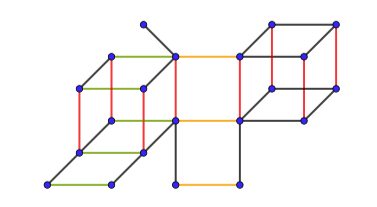
\includegraphics[width=0.6\linewidth]{hyperplane}
        \caption{The yellow hyperplane separates two halfspaces in the left and in the right.}
    \end{figure}
    
     One should keep in mind that hyperplanes in fact capture the geometry of median graphs, motivated by the following theorem:
    
    \begin{theorem}[\cite{genevois}]
        In a median graph, the following facts hold:
        
        \begin{enumerate}
            \item Every hyperplane delimits exactly two halfspaces.
            \item Carriers and halfspaces are convex.
            \item A path is a geodesic if and only if it crosses each hyperplane at most once.
            \item The distance between two vertices coincides with the number of hyperplanes separating them.
        \end{enumerate}
    \end{theorem}
    
    \section{Equivalence of median graphs and CAT(0)-cube complexes}
    
    In this last section, we will present the following theorem, which is the core of this talk:
    
    \begin{theorem}[\cite{hagen}]
        Let $X$ be a CAT(0) cube complex, then
        
        \begin{enumerate}
            \item $X^{(1)}$ is a median graph.
            \item If $Y \subset X$ is a cubically convex subcomplex, then $Y^{(1)}$ is a median-convex subgraph of $X^{(1)}$.
            \item If $Y \subset X$ is a full subcomplex of $X$ and $Y^{(1)}$ is median-convex in $X^{(1)}$, then $Y$ is a convex subcomplex.
            \item For each hyperplane $H$ of $X$, due to an edge $e$, the convex split $\overleftarrow{e}$ and $\overrightarrow{e}$ is exactly the partition of $X^{(0)}$ induced by the two components of $X \setminus H$.
        \end{enumerate}
        
        Conversely:
        
        \begin{enumerate}
            \item If $G$ is a median graph, then there exists a unique CAT(0) cube complex $X$, such that $X^{(1)} \cong G$.
            \item If $H \subset G$ is a median-convex subgraph, then the CAT(0) cube complex $Y$ with $1$-skeleton $H$ is a convex subcomplex of $X$, spanned by $H$.
        \end{enumerate}
    \end{theorem}
    
    We first would like to show that $1$-skeleta of CAT(0) cube complexes are median:
    
    \begin{lemma}
        If $X$ is a CAT(0) cube complex, then $X^{(1)}$ is a median graph.
    \end{lemma}
    
    \begin{proof}
        We may arbitrarily pick three vertices $x$, $y$, and $z$ from $X$. Let $H$ be a hyperplane, and $\overleftarrow{H}$ and $\overrightarrow{H}$ are the associated halfspaces. Without loss of generality, we can say that $\overleftarrow{H}$ contains at least two of the three vertices, by the pigeonhole principle.
        
        We may let $S$ be the set of halfspaces, as $H$ varies over all the hyperplanes. Notice that for each hyperplane, $S$ contains exactly one halfspace.
        
        We also notice that if $H$ and $H'$ are two halfspaces, then both $\overleftarrow{H}$ and $\overrightarrow{H'}$ contain at least two of the vertices from the three-vertex set ${ x, y, z}$, again, by the pigeonhole principle.
        
        If $S_{x}$ is the set of halfspaces containing $x$, then any hyperplane $H$ separates $x$ from both $y$ and $z$ such that $x \notin \overleftarrow{H}$, so $\abs{S - S_{x}} \leq d_{1}(x, y) + d_{1}(x, z)$. By Lemma 1.12 from \cite{hagen}, we know that there exists a unique $m \in X^{(0)}$, such that $S_{m} = S$.
        
    \end{proof}
    
    \nocite{*}
    \bibliographystyle{plain}
    \bibliography{biblio}
    
\end{document}
